

% Gradient Info
  
\tikzset {_f6md6ajgy/.code = {\pgfsetadditionalshadetransform{ \pgftransformshift{\pgfpoint{0 bp } { 0 bp }  }  \pgftransformscale{1 }  }}}
\pgfdeclareradialshading{_jk0eqd11o}{\pgfpoint{0bp}{0bp}}{rgb(0bp)=(0.97,0.91,0.11);
rgb(0bp)=(0.97,0.91,0.11);
rgb(25bp)=(1,1,1);
rgb(400bp)=(1,1,1)}
\tikzset{every picture/.style={line width=0.75pt}} %set default line width to 0.75pt        

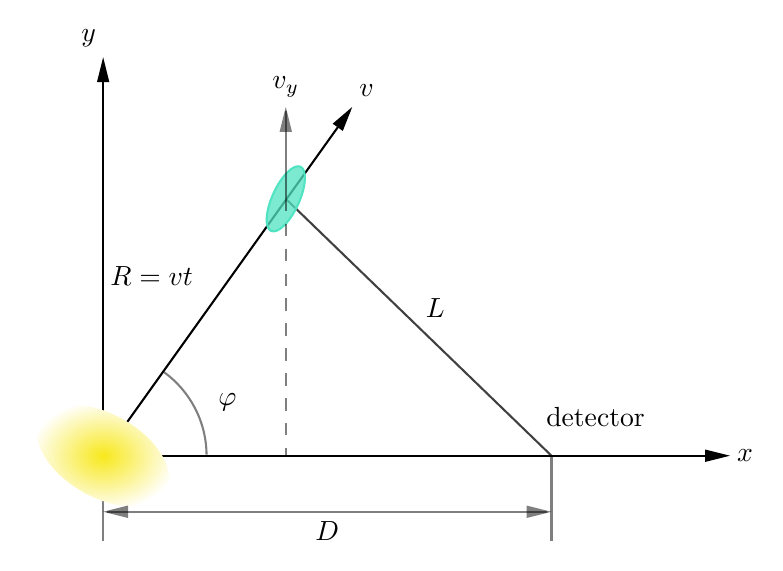
\begin{tikzpicture}[x=0.75pt,y=0.75pt,yscale=-1,xscale=1]
%uncomment if require: \path (0,315); %set diagram left start at 0, and has height of 315

%Straight Lines [id:da8791392372886593] 
\draw [color={rgb, 255:red, 0; green, 0; blue, 0 }  ,draw opacity=0.75 ]   (184,118.23) -- (312,242) ;
%Straight Lines [id:da6990399911927212] 
\draw [color={rgb, 255:red, 0; green, 0; blue, 0 }  ,draw opacity=0.5 ]   (96,242) -- (96,283) ;
%Straight Lines [id:da929753289055431] 
\draw [color={rgb, 255:red, 0; green, 0; blue, 0 }  ,draw opacity=1 ]   (96,242) -- (214.84,75.63) ;
\draw [shift={(216,74)}, rotate = 125.54] [fill={rgb, 255:red, 0; green, 0; blue, 0 }  ,fill opacity=1 ][line width=0.08]  [draw opacity=0] (12,-3) -- (0,0) -- (12,3) -- cycle    ;
%Straight Lines [id:da9476652899394022] 
\draw    (96,242) -- (396,242) ;
\draw [shift={(398,242)}, rotate = 180] [fill={rgb, 255:red, 0; green, 0; blue, 0 }  ][line width=0.08]  [draw opacity=0] (12,-3) -- (0,0) -- (12,3) -- cycle    ;
%Straight Lines [id:da12075393106418608] 
\draw    (96,242) -- (96,52) ;
\draw [shift={(96,50)}, rotate = 90] [fill={rgb, 255:red, 0; green, 0; blue, 0 }  ][line width=0.08]  [draw opacity=0] (12,-3) -- (0,0) -- (12,3) -- cycle    ;
%Shape: Ellipse [id:dp7501822937817628] 
\draw  [draw opacity=0][shading=_jk0eqd11o,_f6md6ajgy] (65.63,224.61) .. controls (71.12,215.02) and (89.17,215.04) .. (105.94,224.64) .. controls (122.71,234.25) and (131.86,249.81) .. (126.37,259.39) .. controls (120.88,268.98) and (102.83,268.96) .. (86.06,259.36) .. controls (69.29,249.75) and (60.14,234.19) .. (65.63,224.61) -- cycle ;
%Shape: Arc [id:dp14808297636810597] 
\draw  [draw opacity=0] (125.4,201.77) .. controls (137.65,210.74) and (145.66,225.17) .. (145.82,241.5) -- (96,242) -- cycle ; \draw  [color={rgb, 255:red, 0; green, 0; blue, 0 }  ,draw opacity=0.5 ] (125.4,201.77) .. controls (137.65,210.74) and (145.66,225.17) .. (145.82,241.5) ;
%Shape: Ellipse [id:dp5550484242786045] 
\draw  [color={rgb, 255:red, 80; green, 227; blue, 194 }  ,draw opacity=1 ][fill={rgb, 255:red, 80; green, 227; blue, 194 }  ,fill opacity=0.75 ] (191.07,102.77) .. controls (187.81,101.28) and (181.99,106.99) .. (178.09,115.53) .. controls (174.18,124.06) and (173.66,132.2) .. (176.93,133.69) .. controls (180.19,135.18) and (186.01,129.47) .. (189.91,120.93) .. controls (193.82,112.39) and (194.34,104.26) .. (191.07,102.77) -- cycle ;
%Straight Lines [id:da06332288321674429] 
\draw [color={rgb, 255:red, 0; green, 0; blue, 0 }  ,draw opacity=0.5 ]   (312,242) -- (312,283) ;
%Straight Lines [id:da6458514363662675] 
\draw [color={rgb, 255:red, 0; green, 0; blue, 0 }  ,draw opacity=0.5 ]   (98,269) -- (310,269) ;
\draw [shift={(312,269)}, rotate = 180] [fill={rgb, 255:red, 0; green, 0; blue, 0 }  ,fill opacity=0.5 ][line width=0.08]  [draw opacity=0] (12,-3) -- (0,0) -- (12,3) -- cycle    ;
\draw [shift={(96,269)}, rotate = 0] [fill={rgb, 255:red, 0; green, 0; blue, 0 }  ,fill opacity=0.5 ][line width=0.08]  [draw opacity=0] (12,-3) -- (0,0) -- (12,3) -- cycle    ;
%Straight Lines [id:da4496754806264811] 
\draw [color={rgb, 255:red, 0; green, 0; blue, 0 }  ,draw opacity=0.5 ] [dash pattern={on 4.5pt off 4.5pt}]  (184,118.23) -- (184,242) ;
%Straight Lines [id:da29868680463289254] 
\draw [color={rgb, 255:red, 0; green, 0; blue, 0 }  ,draw opacity=0.5 ]   (184,76) -- (184,118.23) ;
\draw [shift={(184,74)}, rotate = 90] [fill={rgb, 255:red, 0; green, 0; blue, 0 }  ,fill opacity=0.5 ][line width=0.08]  [draw opacity=0] (12,-3) -- (0,0) -- (12,3) -- cycle    ;

% Text Node
\draw (400,242) node [anchor=west] [inner sep=0.75pt]    {$x$};
% Text Node
\draw (94,46.6) node [anchor=south east] [inner sep=0.75pt]    {$y$};
% Text Node
\draw (150,210.4) node [anchor=north west][inner sep=0.75pt]    {$\varphi $};
% Text Node
\draw (204,272.4) node [anchor=north] [inner sep=0.75pt]    {$D$};
% Text Node
\draw (250,176.71) node [anchor=south west] [inner sep=0.75pt]    {$L$};
% Text Node
\draw (98,149.4) node [anchor=north west][inner sep=0.75pt]    {$R=vt$};
% Text Node
\draw (218,70.6) node [anchor=south west] [inner sep=0.75pt]    {$v$};
% Text Node
\draw (184,70.6) node [anchor=south] [inner sep=0.75pt]    {$v_{y}$};
% Text Node
\draw (308,217) node [anchor=north west][inner sep=0.75pt]   [align=left] {detector};


\end{tikzpicture}
